\chapter{Background}
\label{cha:background}
This thesis investigates a middleware for de-identifying data exposed through the Solid protocol. Section \ref{sec:solid} introduces the basic concepts of Solid, while section \ref{sec:pets} introduces some necessary background knowledge on Privacy-Enhancing Technologies (PETs).

\section{Solid}
\label{sec:solid}

\subsection{Introduction}
\begin{quote}{Tim Berners-Lee}
    The Semantic Web is not a separate Web but an extension of the current one, in which information is given well-defined meaning, better enabling computers and people to work in cooperation.
\end{quote}

\noindent In 2001, Sir Tim Berners-Lee - the inventor of the world-wide web - published an article in \textit{Scientific American} entitled `The semantic Web' \citep{semantic-web}. It envisioned a future where the Web was not just a collection of pages with meaningless links to each other, but a smart Web, where objects have well-defined meanings.

Today, most resources accessible on the Web are meant for people to read, understand and process, but it is not adapted to automated processing by software agents. Computers can read information and format it correctly, but they lack a unified way to interpret the information: there is no way to process the \textit{semantics}. The Semantic Web tries to solve this problem by extending the current Web with new, compatible standards and protocols to attach computer-readable meaning to information available on the Web.

Currently, XML enables users to arbitrarily structure documents the way they want it (e.g. using a tag called \texttt{<book>} and a tag called \texttt{<isbn>}) and they then write software that parses this by telling the software that \texttt{<book>} means "book" and \texttt{<isbn>} means "isbn". However, other users may use different terms (e.g. \texttt{<livre>}), making information not universally parsable. 

\noindent The Semantic Web introduces RDF\footnote{Resource Description Framework}, which encodes structure and information in sets of triples: similar to a subject, a verb and an object. They are all identified by a URI, making them universal, and allowing anyone to define new verbs. Like this, webs of information are formed between related objects using definitions that can be found and understood by everyone.

This does not completely solve the problem, however. It is possible that multiple definitions exist for essentially the same object. To resolve this, the Semantic Web introduces a third component: ontologies. Ontologies are documents that formally define the relations among terms \citep{semantic-web}. A widely-used ontology is called \textit{foaf}\footnote{\url{ http://xmlns.com/foaf/spec/}} (friend-of-a-friend): it is used to describe relationships between people.


\subsection{The Solid Protocol}
\begin{quote}{\href{https://solidproject.org}{solidproject.org}}
    Solid is a proposed set of conventions and tools for building \textit{decentralized applications} based on Linked Data principles.
\end{quote}
\noindent Solid \citep{solid} is a proposed W3C specification that wishes to decentralize the web by giving people control over their data. Solid aims to realize this by giving people an online datastore called a pod. Users can then login to applications using an authentication mechanism provided by Solid, and the application can in turn access data stored in the user's pod.

By storing all the data inside the user's pod instead of on the application server, the user retains complete control over his data. He can flexibly choose what data to share with what applications. Furthermore, storing the data in a pod reduces vendor lock-in: when the user wishes to switch from one service to another, he can simply give the new application access to the data he already possesses. 
In Solid, there are two types of resources: linked and non-linked data resources. Non-linked data resources are the usual kinds of data that we access on the web right now (binary, text, images, ...), while linked data follows the 
 RDF specifications by using a content representation such as Turtle \citep{turtle}. These linked-data standards follow the principles of the Semantic Web.

\subsection{Authentication}
Authenticating a user is the act of verifying a user's claimed identity. Identities in solid (both for users and other agents) follow the WebID standard \citep{webid}: URIs act as universal identifiers. An example WebID is:

\begin{center}
   \texttt{https://jessegeens.solidcommunity.net/profile/card\#me}\\
\end{center}

\noindent These WebID URIs can identify several things: users, software agents, or other things (even if they do not exist on the web). The WebID URI references a WebID Profile Document. This document contains information about the agent who is the referent of the WebID URI. However, an important distinction must be made. When the \textit{\texttt{\#me}} is included in the URI (or more in general, the hashtag), this URI refers to an agent. When the hashtag is omitted, the URI refers to the document describing this agent.

While the WebID standard provides identities, it does not yet verify them. The actual authentication (or, verifying that the agent actually controls the WebID he claims to control) in Solid uses the WebID-OIDC protocol. This protocol draws inspiration from OAuth2 and from OpenID Connect. The below workflow, drawn from the WebID-OIDC repository, explains the basic mechanism of the protocol:

\begin{quote}{\href{https://github.com/solid/webid-oidc-spec}{webid-oidc-spec repository}}

    1. \textbf{Initial Request}: Alice (unauthenticated) makes a request to bob.example, receives a \texttt{HTTP 401 Unauthorized} response, and is presented with a 'Sign In With...' screen.\\
    
    2. \textbf{Provider Selection}: She selects her WebID service provider by clicking on a logo, typing in a URI (for example, alice.solidtest.space), or entering her email.\\
    
    3. \textbf{Local Authentication}: Alice gets redirected towards her service provider's own Sign In page, thus requesting https://alice.solidtest.space/signin, and authenticates using her preferred method (password, WebID-TLS certificate, FIDO 2 / WebAuthn device, etc).\\
    
    4. \textbf{User Consent}: (Optional) She's presented with a user consent screen, along the lines of "Do you wish to sign in to bob.example?".\\
    
    5. \textbf{Authentication Response}: She then gets redirected back towards https://bob.example/resource1 (the resource she was originally trying to request). The server, bob.example, also receives a signed ID Token from alice.solidtest.space that was returned with the response in point 3, attesting that she has signed in.\\
    
    6. \textbf{Deriving a WebID URI}: bob.example (the server controlling the resource) validates the ID Token, and extracts Alice's WebID URI from inside it. She is now signed in to bob.example as user https://alice.solidtest.space/\#i.\\
    
    7. \textbf{WebID Provider Confirmation}: bob.example confirms that solidtest.space is indeed Alice's authorized OIDC provider (by matching the provider URI from the iss claim with Alice's WebID).

\end{quote}

\subsection{Authorization}
Authorization within the Solid project builds on the Web Access Control standard \citep{wac}. The WAC standard provides a method to define authorization conditions for resources in a Pod using an Access Control List. Every resource is coupled with an ACL resource - either directly, or by inheriting it from a parent container. These ACL resources are using the ACL ontology, usually in a turtle file\footnote{Other RDF representations are also allowed, but support for turtle files is mandatory}. Authorization conditions consist of three elements: access objects (the associated resource), access modes (\textit{read}, \textit{write}, \textit{append} or \textit{control}) and access subjects (the agents performing the request).

The access objects in an ACL resource are the resources the ACL resource refers to. This can be both a normal resource (LDP-RS or LDP-NR, see \ref{subsec:ldp}) as well as a container. It is not mandatory for resources to have an associated ACL resource, as these can be inherited. This mechanism ensures that there is no need to create duplicate ACL resources for similar resources, as well as ensuring proper protection for newly created resources. When a resource is accessed, the server will first look for a directly associated ACL resource. When none is found, the server will walk up the container tree (starting from the current container the resource is located in, then the parents, up until the root container). Once an ACL resource applying to one of the parent containers is found, this is applied to the requested resource.

Possible access modes, then, are either \textit{read}, \textit{write}, \textit{append} or \textit{control}. Reading and writing are the usual operations. Append is a subset of writing: data can be added to the resource, but not deleted. This is useful for, for example, logging applications, ensuring that logs cannot be removed. Since appending is a subset of writing, the writing authorization implies the appending authorization (no resource can allow writing but disallow appending). Finally, control means being able to modify the ACL of the resource. Being able to control a resource generally implies ownership of the resource.

Lastly, access subjects are those agents who request a certain operation on the resource. Generally, these can be divided into four categories. The first one is \textit{every agent}, i.e., the resource is publicly accessible. A second option is authenticated agents only (with no restrictions on who these agents are), which may be useful for auditing purposes. Thirdly, resource access can be restricted to agents with a specific WebID. Finally, this can also be extended to groups of agents (where the group has a single WebID).

An example ACL resource, taken from the Solid Community Server\footnote{See \url{https://github.com/solid/community-server}}, is presented below:
\lstinputlisting[style=turtle, title=.acl, caption=Access Control List Resource]{code/acl.ttl}

\subsection{Linked Data Platform and Containers}
\label{subsec:ldp}
Solid mainly relies on the LDP protocol \citep{ldp} for resource management. The LDP protocol uses HTTP for accessing and modifying resources on a server. LDP Resources, or LDPRs, are HTTP resources that conform to a number of conventions. There are multiple types of resources:
\begin{enumerate}
    \item RDF Sources, also called LDP-RSs (LDP RDF Source)
    \item Non-RDF Sources, such as images or binary data, which are called LDP-NRs
    \item Containers, a concept for bundling related resources together. These are also called LDPCs (LDP Container). 
\end{enumerate}

\noindent To support the access and modification of these resources, LDP servers must support a number of HTTP methods on the resources. The \texttt{GET} method is mandatory and returns the request resource, if certain conditions are met (e.g., does the agent have the correct authorizations to access the resource). The \texttt{POST} and \texttt{PUT} methods are optional, and allow agents to create new resources or modify existing ones. Similarly, the \texttt{DELETE} method is optional and allows agents to delete resources. The \texttt{HEAD} and \texttt{OPTIONS} methods are mandatory to be implemented by servers and are similar to the methods defined in the HTTP/1.1 protocol. Below is an example of a request for a basic container and the accompanying reply \citep{ldp-primer}:

\begin{verbatim}
GET /alice/ HTTP/1.1
Host: example.org
Accept: text/turtle
HTTP/1.1 200 OK 
Content-Type: text/turtle; charset=UTF-8
Link: <http://www.w3.org/ns/ldp#BasicContainer>; rel="type", 
      <http://www.w3.org/ns/ldp#Resource>; rel="type"
Allow: OPTIONS,HEAD,GET,POST,PUT,PATCH
Accept-Post: text/turtle, application/ld+json, image/bmp, image/jpeg
Accept-Patch: text/ldpatch
Content-Length: 250
ETag: W/'123456789'
	
@prefix dcterms: <http://purl.org/dc/terms/>.
@prefix ldp: <http://www.w3.org/ns/ldp#>.
	
<http://example.org/alice/> a ldp:Container, ldp:BasicContainer;
  dcterms:title 'Alice`s data storage on the Web' .	
\end{verbatim}

\begin{formal}
\textbf{Optional reading} $ - $
\textit{LDP Containers}\\

\noindent LDP Containers are a specialization of a LDP RDF Source, which represent a set of links to other LDPRs that are contained within the container. There are multiple types of LDPCs. The simplest one is the Basic Container or LDP-BC. It defines a basic notion of containment using a generic vocabulary and a \texttt{ldp:contains} relationship. In LDP-BCs, there are no restrictions on LDPRs contained within. The figure below illustrates a LDP Basic Container.\\
\phantom{kkkkkkkkk||||||}{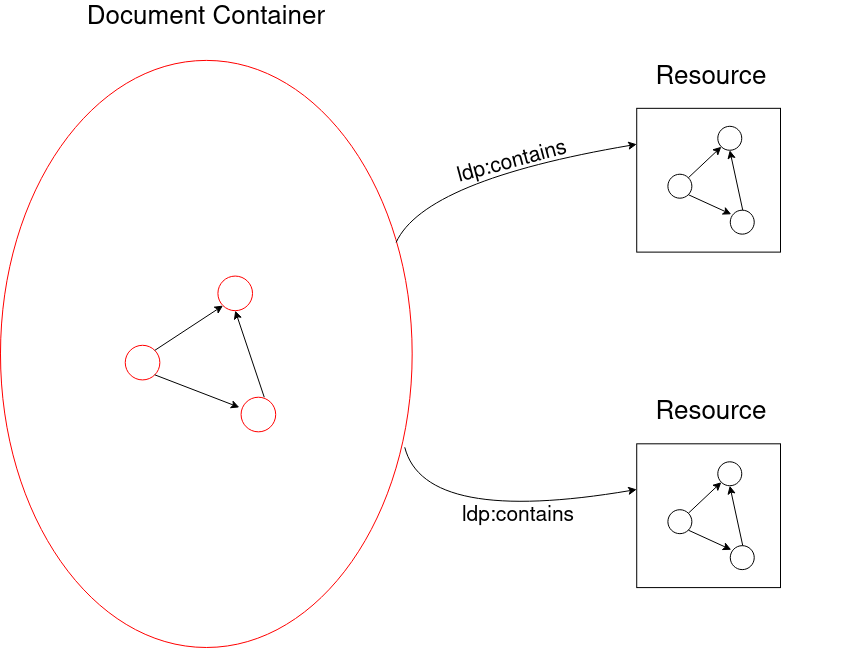
\includegraphics[width=0.60\textwidth]{images/background/ldp-bc.png}}\\
\noindent Direct Containers, or LDP-DCs, are a specialization of a Basic Container. The LDP-DC can make assertions, called membership triples, on resources withing the container. These assertions, which use domain-specific vocabulary, are made as part of the creation process for resources placed in the container. The membership triples do not need to refer to the container resource - these can refer to other resources as well. The figure below illustrates a LDP Basic Container containing movies, and a LDP Direct Container containing documents (images, movies, ..) where the actor is depicted, illustrated through the verb \texttt{foaf:depicton}. \\
\phantom{kkkkkk|||}{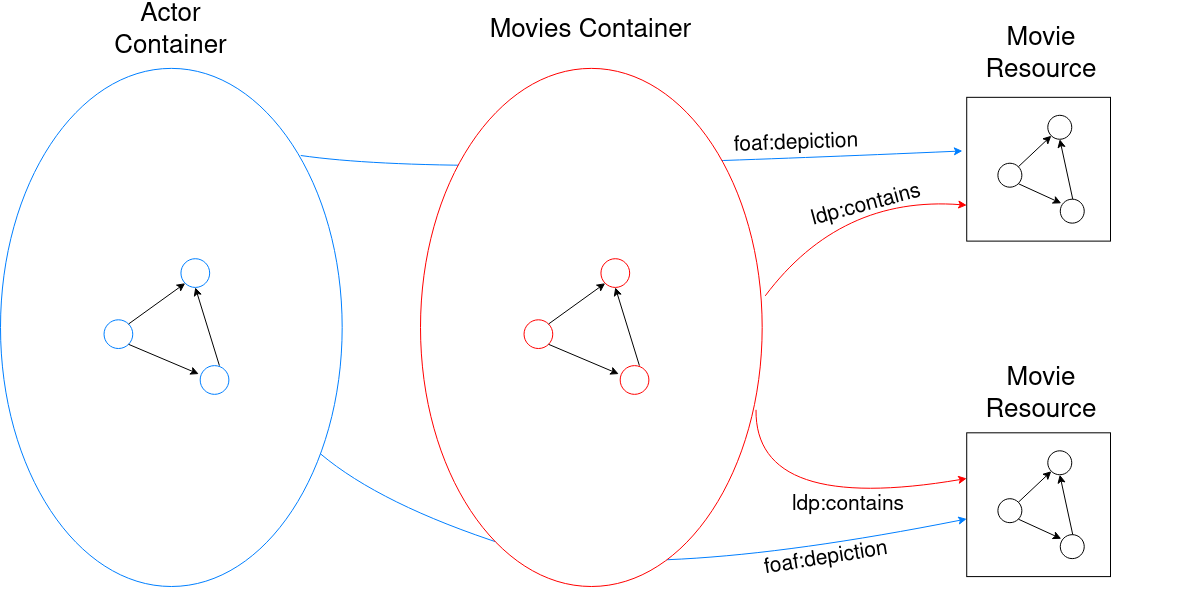
\includegraphics[width=0.8\textwidth]{images/background/ldp-dc.png}}\\

\noindent \textit{Source}: \url{https://www.w3.org/TR/ldp-primer/}
\end{formal}

\section{Privacy-Enhancing Technologies}
\subsection{The need for Privacy-Enhancing Technologies}
The concept of privacy has been around for a long time. Even in the 14th century already, cases were brought before court for eavesdropping and opening letters \citep{privacy-history}. Initially, it was more understood in the context of being let alone, especially in one's house or personal properties. Since the dawn of the information age after the Second World War, the concept started to shift more towards privacy in the context of personal information and publications on the topic started to appear. The definition did not change much however, remaining very similar to the one introduced in 1891 by Warren and Brandeis \citep{privacy-history}:
\begin{quote}{Samuel Warren, Louis Brandeis}
    Privacy is described as a right to be let alone and a right of each individual  to  determine,  under  ordinary  circumstances,  what  his  or  her  thoughts, sentiments, and emotions shall be when in communication with others.
\end{quote}
The ubiquity of personal data collection in recent years has strengthened privacy concerns. Especially since the Web has become extremely centralized, with only a six companies accounting for 43\% of global internet traffic \citep{internet-report}, there has been a growing demand for technologies that help protect user privacy.

Not only from the data subject's perspective is there a growing concern for data privacy. With the introduction of the General Data Protection Regulation (GDPR) in 2018, companies have a legal obligation to take care of user data, especially if it is sensitive. This clashes with the rise of the Saas/PaaS business models, where companies outsource data storage and management. However, this is not always possible and comes with risks. If a Data Processor (a third party that processes data on behalf of a Data Controller) leaks data, the Data Owner risks violating the user's trust (and legal sanctions). 

In both cases, Privacy-Enhancing Technologies play a big role in reducing the risk of data leaks and preserving user privacy. \citeauthor{pets-handbook} introduced the following definition, which was later adopted by the European Commission\footnote{\url{https://eur-lex.europa.eu/LexUriServ/LexUriServ.do?uri=COM:2007:0228:FIN:EN:PDF}}:

\begin{quote}{\citeauthor{pets-handbook}}
    Privacy-Enhancing Technologies is a system of ICT measures protecting informational privacy by eliminating or minimising personal data thereby preventing unnecessary or unwanted processing of personal data, without the loss of the functionality of the information system.
\end{quote} 

\todo{Write paragraph here about the importance of taking privacy into account at the onset of software design, inspired by Van Landuyt and Hoepman}

The following sections will introduce a number of widely used PETs, some of which will be used in the middleware.\todo{vervangen door naam middleware}

\subsection{Data (de-)identification}
\todo[inline]{use this section to introduce definitions for PII, explain direct and indirect identifiers, introduce some GDPR terms like processor and subject etc -> name "privacy by design"!}

\subsection{Transformation-based Approaches}
Transformation-based approaches are approaches that modify datasets in a uniform way, such that the resulting dataset contains less personally identifiable information (PII). Since data transformations \textit{modify} the dataset, it is important to note that this has an impact on the utility of the data. Some transformations may be more powerful at anonymizing the data, but at the same time make the data less valuable or even unusable. A balance must be struck between data privacy and utility, where the choice for a certain data transformation is very context-dependant. This section introduces a number of data transformations.

\subsection{Encrypted Database Systems}
\subsection{Other Approaches}
\subsubsection{Multi-Party Computation}
\subsubsection{Differential Privacy \& \textit{k}-Anonymity}
\label{sec:pets}